\documentclass[12pt,a4paper]{report}

\usepackage{enumitem}
\usepackage[utf8x]{inputenc}
\usepackage[francais]{babel}
\usepackage[T1]{fontenc}
\usepackage{amsmath}
\usepackage{amsfonts}
\usepackage{amssymb}
\usepackage[square,sort,comma,numbers]{natbib}
\usepackage[colorlinks=true,linkcolor=blue]{hyperref}
\usepackage{glossaries}
\usepackage[usenames,dvipsnames]{xcolor}
\usepackage{setspace}
\usepackage{graphicx}
\usepackage[rightcaption]{sidecap}
\usepackage{subfigure}
\usepackage{float}
\usepackage[skip=2pt,font=scriptsize]{caption}
\usepackage{listings}
\usepackage{xcolor}
\usepackage[top=2cm, bottom=3cm, left=2cm , right=2cm]{geometry}

\author{Nicolas JEANNE}
\title{Rapport de stage de M2}
\date{11 mars 2015}

% Mise en page des citations
\bibliographystyle{abbrvnat}
\setcitestyle{authoryear,open={(},close={)},aysep={},citesep={;}}


% formattage des entrées du glossaire
%\renewcommand*{\glstextformat}[1]{\emph{#1}}
% création des acronymes du glossaire
\newacronym{rep}{REP}{Repeated Extragenic Palindrome}
\newacronym{bime}{BIME}{Bacterial Interspesed Mosaic Element}
\newacronym{sra}{SRA}{Sequence Read Archive}
\newacronym{ngs}{NGS}{Next Generation Sequencing}
\newacronym{sam}{SAM}{Sequence Alignment Map format}
\newacronym{bam}{BAM}{Binary Alignment Map format}
\newacronym{gff}{GFF}{General Feature Format}
\newacronym{bed}{BED}{Browser Extensible Data}
\newacronym{de}{DE}{Diff\'erence d'Expression}
\newacronym{rpkm}{RPKM}{Reads Per Kilobase per Million mapped reads}
\newacronym{pdp}{PDP}{Pruned Dynamic Programming}
% création des entrées du glossaire
\newglossaryentry{PE}{name={Paired-end sequencing},description={Technique de séquençage haut débit consistant à réaliser les amplifications d'un fragment d'ADN en marquant l'extrémité 5' par un tag \no1 et l'extrémité 3' par un tag \no2. La distance entre les 2 tags est connue et fixe (négative ou jusqu'à 500 pb). Ceci permet lors de l'assemblage, de séquences de 35 pb par exemple, d'associer le read 1 et le read 2 grâce à la distance séparant les 2 et cela même si la séquence intermédiaire est inconnue. Si la distance est négative, il est possible d'obtenir des reads chevauchants de longueur plus importante que les 35 pb}}
\newglossaryentry{SE}{name={Single-end sequencing},description={Technique de séquençage haut débit la plus simple consistant à ne réaliser le séquençage que depuis une extrémité du template.}}
\newglossaryentry{reads}{name={reads},description={Séquence nucléotidique issue d'un séquençage NGS}}
\newglossaryentry{GRanges}{name={Genomic Ranges},description={Format de stockage d'informations pour les éléments génomiques sous R. L'information minimale requise est le chromosome, les positions de départ et de fin, le sens du brin. Ces champs peuvent être suivis de méta-datas où d'autres informations libres peuvent être enregistrées}}
\newglossaryentry{chimerique}{name={alignement chim\'erique},description={L'alignement d'un read ne peut pas être représenté comme un alignement linéaire. Un alignement chimérique est représenté comme un ensemble d'alignements, par exemple lorsqu'une partie d'un read est mappé à un locus du génome et la suite à un autre locus}}
\newglossaryentry{couverture}{name={couverture},description={Appelé également profondeur de séquençage, correspond au nombre de reads alignés sur une région génomique. Dans le cas du RNAseq, la couverture fournit une information sur le taux d'expression d'un élément génomique}}
\newglossaryentry{nb}{name={loi Binomiale N\'egative },description={Si une expérience consiste en une série de tirages indépendants  avec une probabilité de succès $p$ et une probabilité d'échec complémentaire, celle-ci se poursuit jusqu'à l'obtention de $n$ succès, la variable aléatoire représentant le nombre d'échecs avant l'obtention des $n$ succès suit une loi négative binomiale. Les paramètres de cette loi sont $n$ le nombre de succès attendus et $p$ la probabilité d'un succès}}
\makeglossaries

% Encadrement des figures
\floatstyle{boxed}
\restylefloat{figure}

% Configuration des liens
\hypersetup{
  colorlinks,
  citecolor=Violet,
  linkcolor=Black,
  urlcolor=Blue}

% Configuration des parties de code
\lstset{basicstyle=\small}

\begin{document}

\maketitle

\begin{onehalfspace}
\chapter*{Introduction}
En 1982, la découverte par Higgins de nouveaux éléments génétiques communs dans les régions intercistroniques des opérons de \textit{Escherichia coli} et \textit{Salmonella typhimurium} a constitué le premier pas de la recherche sur les \gls{rep} \citep{Higgins1982}. En 1991, Gilson et al. ont mis en évidence l'organisation en clusters de ces REP \citep{Gilson1991}. Ces clusters ont été caractérisés comme \gls{bime}. Chez \textit{E. coli} en 1994, Bachelier et son équipe ont réussi à catégoriser les REP constituant les BIME en 2 types Y et Z, constituants 3 motifs Y, Z\textsuperscript{1}, Z\textsuperscript{2}  \citep{Bachellier1994}.
 
Les REP constituent une part non négligeable du génome bactérien, chez \textit{E. coli K12} ou \textit{S. typhimurium} elles représentent environ 1\% de celui-ci \citep{Gilson1991}. Nous les retrouvons chez de nombreux règnes bactériens, notamment chez les pathogènes humains tels que \textit{Escherichia coli, Salmonella enterica, Neisseria meningitidis, Mycobacterium tuberculosis et Pseudomonas aeruginosa} mais également chez des pathogènes des plantes comme \textit{Agrobacterium tumefaciens} ou chez des bactéries ubiquitaires, \textit{Deinococcus radiodurans} ou \textit{Pseudomonas putida} par exemple. Les travaux précédents de l'équipe ont permis l'annotation des REP au sein du génome d'\textit{E. coli} et de mettre en évidence le lien existant entre la prolifération des REP et le gène $tnpA_{REP}$ \citep{Weyder2013,Bosc2014}, ainsi que la reconstruction des états ancêtres des REP \citep{Bosc2014}.  \textcolor{red}{Le rôle exact des REP n'est pas clairement défini, des hypothèses sont avancées sur leur implication dans la régulation de l'expression des gènes, que ce soit en tant que terminateur de transcription ou comme site de reconnaissance des enzymes impliquées dans les mécanismes de la transcription.}

\section*{Caractéristiques des REP et organisations en BIME}

\begin{figure}[ht]
\centerline{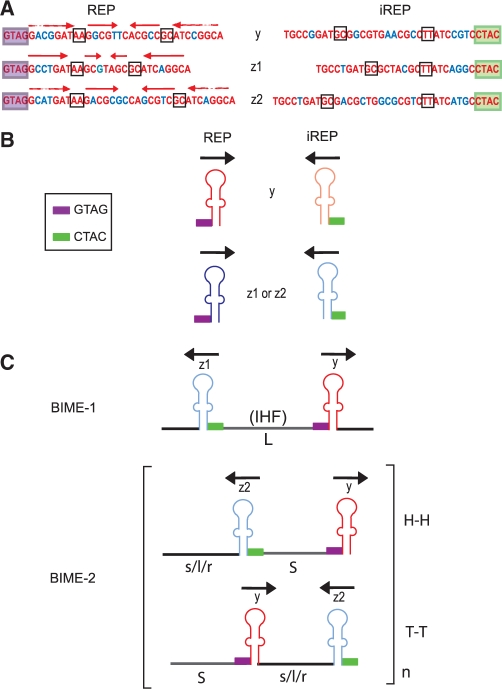
\includegraphics[scale=1.8]{figures/rep_bime.jpg}}
\caption{\textbf{REP et BIME chez \textit{Escherichia coli}. (A)} Séquences consensus Y, Z\textsuperscript{1} et Z\textsuperscript{2} des REP. Le tétra-nucléotide conservé GTAC est encadré en violet, le complémentaire conservé CTAC est encadré en vert, les flèches rouges situent les zones d'appariement de la tige et les positions encadrées en noir sont les zones de mésappariement. Les positions conservées parmi les classes de REP sont en rouge, les positions variables en bleu. \textbf{(B)} Structure secondaire des REP. Les rectangles violets et verts représentent respectivement les tétra-nucléotides conservés GTAC pour les REP et CTAC pour les iREP. Les flèches noires indiquent l'orientation des REP. \textbf{(C)} Structures des BIME-1 et BIME-2. Les BIME-1 sont composées de REP et de iREP Y et Z\textsuperscript{1} séparées par un linker de séquence longue (L), les BIME-2 sont composées de Y et Z\textsuperscript{2}, de linker courts (S) et de séquences séparatrices s, l ou r. H-H et T-T dénotent respectivement une organisation tête à tête et queue à queue des REP. \citep{Ton-Hoang2012}.}
\label{fig:rep_bime} 
\end{figure}

La taille des REP varie de 20 à 40 nucléotides, la classification Y, Z\textsuperscript{1}, Z\textsuperscript{2} est basée à la fois sur la taille de la séquence consensus de la REP ainsi que sur sa structure secondaire. Par convention, une REP en orientation inversée est nommée iREP (inversed REP) \citep{Ton-Hoang2012}. Un tétra-nucléotide caractéristique de séquence GTAC est présent à l'extrémité 5' des REP, sa séquence complémentaire est CTAC en 3' pour les iREP. Les différentes classes de REP partagent des nucléotides conservés (\autoref{fig:rep_bime}A). La structure secondaire des REP est caractérisée par sa forme en tige-boucle, le caractère palindromique permet la formation de la tige malgré un mésappariement situé dans la partie centrale de celle-ci (\autoref{fig:rep_bime}B). Pour le génome d'\textit{E. coli K-12}, 93 REP ont été répertoriées comme étant solitaires sur les 605 annotées par le laboratoire, les autres sont organisées en clusters sous forme de BIME. Une classification a été adoptée comportant 3 entrées, les BIME-1 composées de REP Z\textsuperscript{1} et Y apparaissant en paires uniques dans lesquelles la REP et l'iREP sont séparées par un linker de séquence longue (L) pouvant lier l'IHF (Integration Host Factor). Les BIME-2 constituées de Z\textsuperscript{2} et de Y, apparaissant en copies multiples de cette paire dont la REP et l'iREP sont séparées par un linker court (S) et une des trois séquences flanquantes (s, l ou r). La troisième catégorie est constituée des BIME dites atypiques qui sont des chimères de BIME-1 et BIME-2, comportant différentes combinaisons de Y, Z\textsuperscript{1}, Z\textsuperscript{2}, S, L, s, l et r. Tout comme les BIME-2, nous les retrouvons sous forme de copies multiples (\autoref{fig:rep_bime}C). Les REP peuvent former des structures secondaires avec elles-même, mais également entre elles lorsqu'elles sont organisées sous forme de BIME (\autoref{fig:malEF_rep}).

\begin{figure}[ht]
\centerline{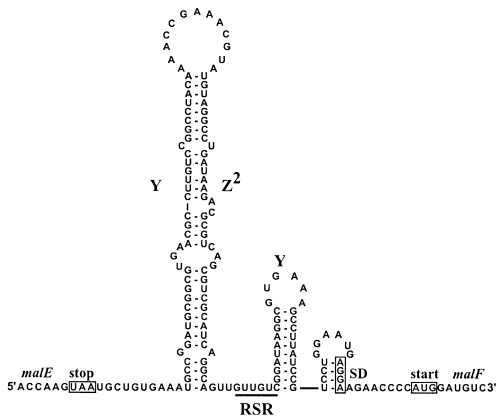
\includegraphics[scale=0.5]{figures/malEF_rep.png}}
\caption{\textbf{Structure ARN des REP au sein de l’opéron malEFG.} Y, Z\textsuperscript{2} et Y indiquent la séquence des REP dans l'espace inter-génique de malE-malF. Bien que Y et Z\textsuperscript{2} puissent former des structures tige-boucles par elles mêmes, elles s'apparient ensemble pour former une région étendue en grande partie à double brin (70\% des nucléotides sont appariés). La séquence affichée provient du génome d'\textit{E. coli K12}. La région REP-stabilized RNA (RSR) indique l'extrémité 3′ du messager malE mature, qui s'étend de 3 à 9 nucléotides depuis la base de la tige-boucle formée par Y et Z\textsuperscript{2}. Les codons STOP de  malE et START de malF sont encadrés. SD représente la séquence Shine–Dalgarno nécessaire à l'initiation de la traduction de malF. \citep{Khemici2004}.}
\label{fig:malEF_rep} 
\end{figure}

\section*{Propriétés associées aux REP}
La littérature décrit de nombreuses fonctions associées aux REP, mais certaines d'entre elles restent encore peu étudiées. Les REP ont été décrite comme jouant un rôle dans les événements de \textbf{recombinaisons homologues} \citep{Kofoid2003}. Les BIME ont été décrites comme des sites privilégiés pour \textbf{l'insertion de séquences d'ADN mobiles} comme certaines familles d'IS (Insertion Sequence) \citep{Bachellier1997,Clement1999,Choi2003,Tobes2005}. Lorsqu'elles sont transcrites, les REP joueraient un rôle dans la \textbf{stabilisation de l'ARNm} grâce à leur structure en tige-boucle \citep{Newbury1987,Espeli2001,Khemici2004,Aguena2009}, la \textbf{terminaison de la transcription} \citep{Gilson1986} et \textbf{le contrôle de la traduction} \citep{Stern1988}. Au niveau de l'ADN, les REP sont capables de \textbf{lier plusieurs facteurs protéiques} tels que l'ADN Gyrase \citep{Espeli1997} et l'ADN polymérase \citep{Gilson1990}. Plus spécifiquement, la BIME-1 peut lier l'\textbf{IHF} sur son linker \citep{Boccard1993} qui peut être notamment responsable de l'\textbf{initiation de la transcription et d’événements de recombinaisons sites spécifiques} \citep{Goosen1995}.

Les propriétés liées à la stabilisation de l'ARNm et la terminaison de la transcription vont nous intéresser plus particulièrement, nous allons nous attacher à décrire ces mécanismes.

\section*{ARN messagers chez \textit{E. coli}}

\subsection*{Stabilité des ARNm}
La dégradation des ARNm chez \textit{E.coli} est réalisée par l'intervention du dégradosome. Il s'agit d'un complexe multi-enzymatique composé de quatre protéines majeures, la RNase E, la PNPase, la RhlB et l'Enolase (\autoref{fig:degradosome}).

\begin{figure}[ht]
\centerline{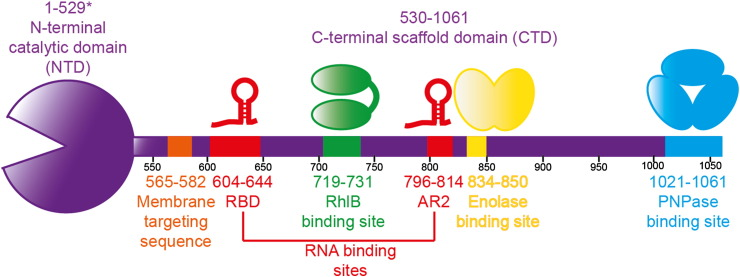
\includegraphics[scale=4]{figures/degradosome.jpg}}
\caption{\textbf{Structure du dégradosome.} Représentation canonique du dégradosome, la partie violette symbolise la RNase E avec le domaine catalytique à gauche, la partie verte le site de liaison de la RhlB, la jaune celui de l'Enolase et la bleue celui de la PNPase \citep{Bandyra2013}.}
\label{fig:degradosome} 
\end{figure}

Un élément clé dans la dégradation du transcrit chez \textit{E. coli} est que celle-ci débute toujours par un clivage réalisé par une endoribonucléase (RNase E). Une fois clivés, les transcrits sont complètement dégradés par des exoribonucléases (RNase R, RNase II ou PNPase) dégradant l'ARNm par l'extrémité 3' et par des oligoribonucléases grâce à la coopération de nombreuses enzymes telles que la poly(A) polymérase (PAP) et les RNA hélicases qui facilitent l'accès aux fragments d'ARN. La RNase E possède une affinité pour les substrats possédant une extrémité mono-phosphate en 5'. Les transcrits primaires bactériens possèdent une extrémité 5' tri-phosphate qui les protège de la dégradation jusqu'à ce qu'ils soient déphosphorylés par l'activité des pyrophosphohydrolases. La RNAse E reconnaît alors l'extrémité 5' mono-phosphate des transcrits par contact de son domaine catalytique \citep{Callaghan2005,Bandyra2013}.

\begin{SCfigure}[][t]
\fbox{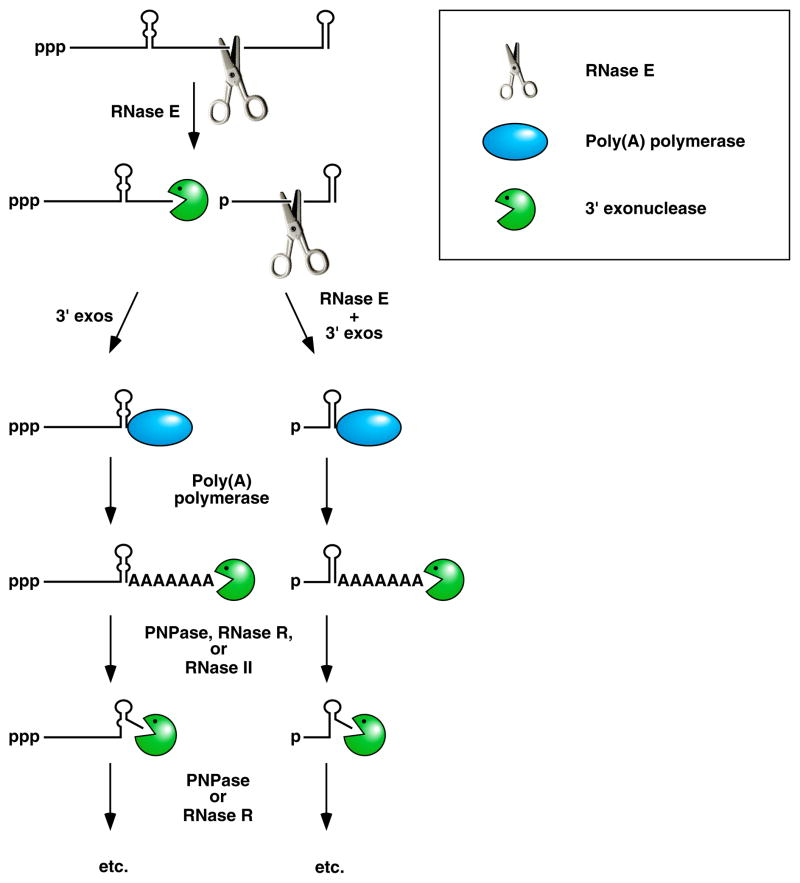
\includegraphics[scale=0.65]{figures/mrna_degradation.jpg}
\caption{\textbf{Facilitation de la dégradation des ARNm chez E. coli par l'intervention de polyadénylation.} Le clivage endonucléolytique par la RNase E génère de multiples fragments, dont certains possèdent à leur extrémité 3' une structure en tige-boucle. Ces fragments subissent une digestion de leur extrémité 3' par la PNPase, la RNase II et/ou la PNPase jusqu'à ce que cette structure soit rencontrée interrompant la dégradation. La PAP intervient pour déstabiliser la tige boucle par l'ajout d'une séquence poly-A en 3' autorisant la reprise de la dégradation par la PNPase et/ou la RNase R \citep{Belasco2010}.}
\label{fig:mrna_degradation} }
\end{SCfigure}

La présence de structure secondaires peut entraver le processus de dégradation initié par les exoribonucléases, la PAP intervient alors en ajoutant sur l'extrémité 3' du transcrit une séquence poly-A qui va déstabiliser la structure secondaire et permettre ainsi aux exoribonucléases de poursuivre la dégradation (\autoref{fig:mrna_degradation}).

\subsection*{Terminaison de la transcription}
Le mécanisme de terminaison de la transcription chez les procaryotes est gouverné par deux classes signaux de fin de transcription. Les terminateurs Rho-dépendant dont l'activité s'appuie sur la liaison de la protéine Rho à un site \emph{rut} (Rho utilization) présent sur le transcrit associé à une interaction avec la RNA Polymérase et les terminateurs Rho-indépendants caractérisés par une structure G-C riche formant une tige-boucle suivie d'une série de résidus U. Ces terminateurs peuvent être bi-directionnels (\autoref{fig:terminator}) \citep{Henkin2000,Lesnik2001}.  

\begin{SCfigure}[][t]
\fbox{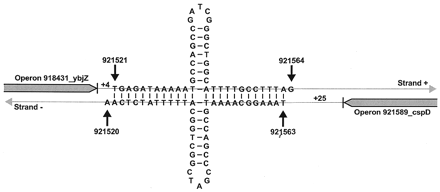
\includegraphics[scale=0.65]{figures/terminator.png}
\caption{\textbf{Terminateur Rho-indépendant bi-directionnel.} La région riche en G-C constitue la structure en tige, la boucle étant formée par les bases non appariées. A la suite de cette structure, nous observons la répétitions de T (U) caractéristique. \citep{Lesnik2001}.}
\label{fig:terminator} }
\end{SCfigure}


\vspace{2.8cm}Les deux aspects de la transcription chez E. coli décrits ci-dessus sont importants car leur caractéristique commune est l'intervention de structures secondaires jouant un rôle dans le processus de dégradation ou de terminaison de la transcription. Pour notre étude ce point est intéressant du fait de la formation de structures secondaires des REP avec elles mêmes ou entre elles qui pourraient jouer un rôle dans la transcription. Nous avons développé des méthodes pour tenter de découvrir le rôle de ces REP en nous basant sur des données d'expressions issues d'expériences de RNA-Seq. 

\chapter*{Matériel \& Méthodes}

\section*{Données}
Plusieurs jeux de données \gls{ngs} ont été utilisés, tous issus d'expériences RNA-Seq publiques, accessibles sur le base de données \href{http://www.ncbi.nlm.nih.gov/geo/}{GEO} (Gene Expression Omnibus) du NCBI au format \gls{sra}. Grâce au \href{http://www.ncbi.nlm.nih.gov/books/NBK158900/#SRA_download.how_do_i_use_the_sra_toolki}{SRA toolkit} et à la commande \texttt{fastq-dump}, elles sont décompressées au format \texttt{fastq}. Un contrôle de qualité est effectué afin d'inspecter les \gls{reads} grâce au logiciel \texttt{fastqc}.

Le \href{http://www.ncbi.nlm.nih.gov/geo/query/acc.cgi?acc=GSE61327}{premier jeu de données} que nous avons exploité est issu des expériences d'évolution adaptatives en laboratoire visant à découvrir l'émergence de mutations clés permettant la croissance rapide d'\textit{E. coli K-12 MG1655} sur un medium pauvre en glucose \citep{Lacroix2014}. Ces données ont été choisies car elles proviennent d'expériences de RNA-Seq comportant un nombre non négligeable de réplicats (9) pour la condition de croissance en milieu pauvre en glucose (ALE) et 2 réplicats pour le Wild Type (WT) , mais nous n'avons exploité que la condition ALE, le nombre de réplicats du WT étant faible. Elles ont été obtenues par séquençage sur Illumina MiSeq à partir d'ARN total extrait des cultures d'\textit{E. coli} et rétro-transcrit en cDNA. La librairie a été conçue en \gls{PE}. 8 réplicats ont été validés puisque disposant d'une qualité de séquence par base supérieure à 30 pour des reads de 62 pb, seul le fichier \texttt{SRR1573441.fastq} a été rejeté car la longueur des reads allait de 35 à 502 pb avec des scores de qualités très variables.

Le \href{http://bioinfolab.uncc.edu/TruHmm_package/raw_data/}{second jeu de données} provient d'une expérience visant à développer un algorithme pour la détection des opérons chez \textit{E. coli K12} \citep{Li2013}. Nous nous sommes intéressés à celles provenant des cultures ayant subi un choc thermique pendant 15 minutes (HS15min) ainsi qu'à celles provenant de culture privées de phosphore pendant 4 heures (M-P4h). Ces 2 conditions ont été retenues car elles possèdent 3 réplicats contre 2 pour toutes les autres. Les librairies ont été conçues en \gls{SE} et brin spécifique en utilisant le kit Illumina’s TruSeq Small RNA Sample Prep, puis séquencées à la fois sur Illumina HiSeq 2000 (générant des reads de 100 bases) et Illumina GA II (générant des reads de 76 bases). Aucun réplicat n'a été rejeté suite aux contrôles qualité.

\section*{Alignement des reads}
Les reads ont été alignés puis mappés sur le génome d'\textit{E. coli} \href{http://www.ncbi.nlm.nih.gov/nuccore/NC_000913.2}{NC\_000913.2}, qui est le génome utilisé pour annoter les REP au laboratoire, grâce au logiciel \href{http://bio-bwa.sourceforge.net/}{BWA}.  Ce logiciel propose 3 algorithmes distincts, BWA-backtrack, BWA-SW et BWA-MEM. Pour chacun de ces alignements, il est nécessaire de disposer de la séquence du génome de référence indexée, obtenue par la commande \texttt{bwa index NC\_000913.2.fasta}. 
L'algorithme que nous avons sélectionné est le MEM (Maximal Exact Matches) pour sa rapidité et sa précision. Il reprend les mêmes principes que BWA-SW (utilisation de la programmation dynamique pour trouver les points d'ancrage (seeds) en autorisant les mésappariements (mismatchs) et les brèches (gaps). Il n'étend les alignements des seeds que lorsque ceux-ci ont peu d'occurrences sur le génome de référence, cela permet de diminuer le temps d'alignement en éliminant les extensions des séquences très répétées) mais en utilisant le seeding avec des MEM, puis il réalise l'extension avec les autorisations de mismatchs et de gaps. Les valeurs par défaut du logiciel ont été utilisées.
\lstset{language=sh, commentstyle=\color{ForestGreen}} 
\begin{lstlisting}[frame=single]
# Alignement avec l'algorithme MEM de BWA
bwa mem ref.fasta file.fastq > aln.sam
\end{lstlisting}
Le fichier d'alignement généré est au format \gls{sam}, afin de poursuivre l'analyse il doit être converti au format \gls{bam}, puis des critères de qualité sont appliqués. Seules les séquences possédant une qualité de mapping > 30 et n'étant pas étiquetées (taggées) comme \gls{chimerique} sont conservées. Cette opération a aussi le mérite de compresser l'information et ainsi de gagner en espace de stockage. Les séquences vont ensuite être triées par position génomique.

Finalement, le fichier BAM trié doit être indexé pour être visualisable sur un Genome Browser. Les outils utilisés sont compris dans la suite des \href{http://samtools.sourceforge.net/samtools.shtml}{samtools}.
\lstset{language=sh, commentstyle=\color{ForestGreen}}  
\begin{lstlisting}[frame=single]
# Conversion du SAM en BAM et application des filtres
# (-q 30: mapping minimal, -F 2048: pas de sequence chimeriques).
samtools view -Sbh -q 30 -F 2048 aln.sam > aln.bam

# Tri en fonction des positions genomiques
samtools sort aln.bam aln_sorted

# Indexation du fichier d'alignement
samtools index aln_sorted.bam
\end{lstlisting}

Pour les besoins ultérieurs de l'analyse, les réplicats d'une même condition sont fusionnés en un seul fichier.
\lstset{language=sh, commentstyle=\color{ForestGreen}}  
\begin{lstlisting}[frame=single]
# Fusion des replicats.
samtools merge merged.bam aln_sorted_1.bam \
aln_sorted_2.bam aln_sorted_3.bam
\end{lstlisting}

\section*{Préparation des fichiers de référence}
Le fichier \gls{gff} d'annotation du génome a été généré par un script Perl à partir du fichier \href{http://www.ncbi.nlm.nih.gov/nuccore/NC_000913.2}{GenBank}. Les fichiers répertoriant les opérons et les promoteurs (source \href{http://regulondb.ccg.unam.mx/}{RegulonDB}), les terminateurs de transcription (source \href{http://csbl.bmb.uga.edu/DOOR/}{Door\up{2}DB}) ainsi que les REP et BIME (source laboratoire) ont été transformés au format \gls{bed} grâce à des scripts Python.
Ces changements de format permettent de travailler aisément avec la suite de logiciels \href{http://bedtools.readthedocs.org/en/latest/}{BEDtools} pour la recherche d'intersections, de positions proches ou de \gls{couverture} de reads. Ces outils ont généré les fichiers \texttt{BED} nécessaires à la suite de l'analyse tel que celui des positions génomiques des opérons contenant des REP, celui des REP, celui des gènes contenus dans des opérons flanquant une REP, celui des BIME et celui de la couverture sur les régions contenant des BIME.

\section*{Visualisation du mapping}
L'alignement des reads et le mapping sur le génome de référence de \textit{E. coli} sont visualisés grâce au genome browser \href{https://www.broadinstitute.org/igv/}{IGV} \citep{Robinson2011,Thorvaldsdottir2013} (\autoref{fig:igv}).

\begin{figure}[ht]
\centerline{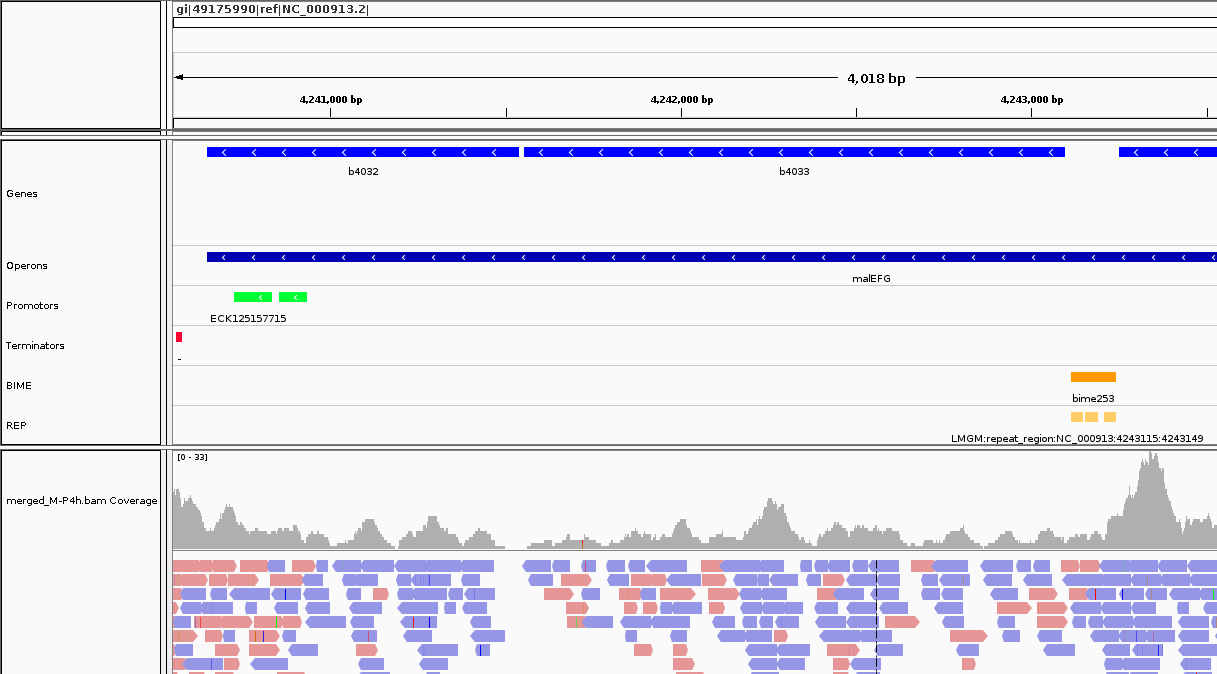
\includegraphics[scale=0.4]{figures/igv_snapshot.png}}
\caption{\textbf{Visualisation du mapping de l'opéron malEFG sur IGV.} Les premières pistes représentent les positions et orientations des gènes, des opérons, la présence de promoteurs et de terminateurs, ainsi que la position des BIME et des REP qui composent les BIME. Les 2 pistes suivantes affichent la couverture des fichiers BAM fusionnés de la région visualisée (histogramme gris) et l'alignement des reads (flèches pleines rouges et bleues). La couleur bleue sur cette piste indique un alignement sur le brin direct et la couleur rouge sur le brin complémentaire.}
\label{fig:igv} 
\end{figure}

Il est important de noter que la couverture le long du génome n'est pas uniforme, ni même sur les gènes, car nous observons la présence de nombreuses vallées et pics. Ce phénomène s'explique par plusieurs raisons techniques \citep{Li2013}. Premièrement, les \textbf{méthodes de fragmentation} des protocoles de préparation des bibliothèques amenant un biais en cassant ou dégradant certaines séquences. Le second biais possible est amené par le \textbf{Random Priming} lors de l'étape de rétro-transcription pouvant préférentiellement transcrire certaines séquences. Troisième point, les \textbf{ligases peuvent lier préférentiellement les adaptateurs} à certaines séquences. Quatrième point, l'amplification de la PCR est bien connue pour introduire des \textbf{biais dépendant de la proportion en GC} des séquences. Le dernier point, étudié sur le séquençage Illumina, implique des \textbf{interférences spécifiques aux séquences} lors du processus d'élongation pendant le séquençage générés par des schémas particuliers du template produisant des repliements du brin d'ADN et altérant l'affinité des enzymes \citep{Nakamura2011}.

\section*{Analyse statistique des données d'expression}
Pour réaliser nos analyses, nous nous sommes inspirés de la méthodologie employée en RNA-Seq pour l'étude de \gls{de}. Il est essentiel de noter qu'une différence importante existe avec notre approche, car \textbf{nous ne nous intéressons pas à une DE pour un m\^eme gène dans différentes conditions mais plutôt à la DE entre deux gènes pour lesquels ont pourrait supposer un profil d'expression similaire dans une même condition}, comme c'est le cas dans les opérons par exemple. L'analyse statistique de recherche de changement d'expression liée à la présence de BIME a été menée sur le logiciel R avec 3 méthodes différentes : la différence d'expression au sein des opérons contenant des BIME, la corrélation de profils et la segmentation.

\subsection*{Création de la table de comptages et normalisation}
Afin d'obtenir des résultats de comptage par région d'intérêt et ainsi estimer l'expression, nous avons utilisé le package Bioconductor easyRNASeq \citep{Delhomme2012} puisqu'il permet de réaliser les opérations de comptage de façon documentée et qu'il offre la possibilité d'effectuer une normalisation par \gls{rpkm}. Les annotations du génome d'\textit{E. coli} relatives aux gènes sont extraites à partir du fichier \texttt{GFF} et stockées sous forme d'une base de données. Cela a nécessité une manipulation préalable de ce fichier, en effet les opérons récupérés sur RegulonDB sont composés à la fois de gènes dont les transcrits sont annotés ARNm, ARNt et ARNr. Seul les gènes dont le transcrit est annoté ARNm est pris en compte par le package easyRNASeq, donc pour ne pas avoir d'erreur dans l'analyse, nous avons transformé les annotations ARNt et ARNr en ARNm.
La liste des transcrits par gène est ensuite extraites pour un total de 4605 éléments que nous nommerons régions. La couverture par région est ensuite calculée pour chaque fichier BAM, le résultat est obtenu en réalisant l'union des positions extraites de la liste des régions et des positions des reads extraites des fichiers BAM qui auront été préalablement transformées au format \gls{GRanges} (GRanges)  \citep{Lawrence2013}. Une table de comptage est alors produite, les régions figurant en ligne et les fichiers BAM en colonnes (\autoref{fig:easyRNAseq}).

\begin{figure}[ht]
\centerline{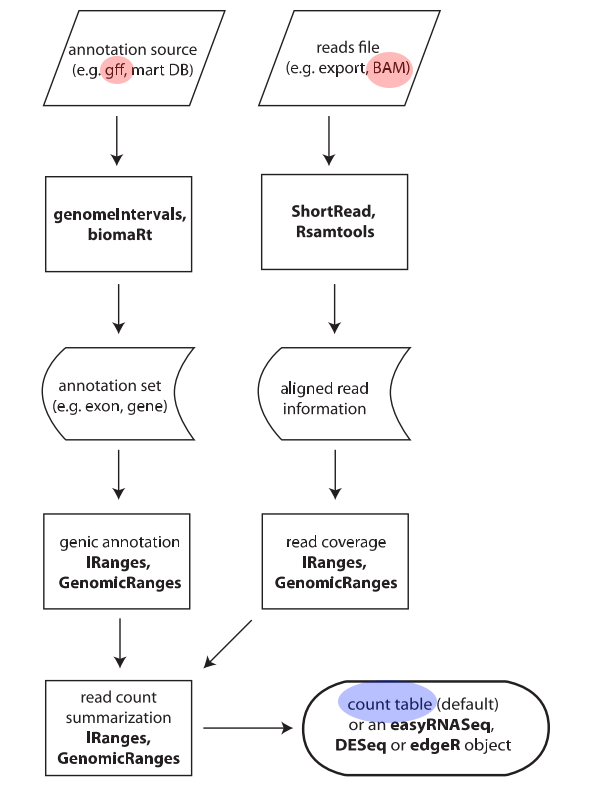
\includegraphics[scale=0.5]{figures/easyRNASeq.png}}
\caption{\textbf{easyRNASeq : création d'une table de comptage.} Processus de création de la table de comptage grâce à l'union des intervalles génomiques. Les formats d'entrées de notre analyse sont surlignés en rouge, le format de sortie en bleu \citep{Delhomme2012}.}
\label{fig:easyRNAseq} 
\end{figure}

Les résultats de comptages doivent ensuite être normalisés afin de permettre la comparaison de l'expression des gènes et des régions génomiques d'intérêt. Notre choix s'est porté sur la méthode du RPKM \citep{Mortazavi2008} :

\[RPKM = Nb.~reads~transcrit~*~\frac{1000~bases~*~10^6}{Nb.~total~reads~*~Taille~du~transcrit}\]

Le RPKM reflète la concentration molaire du transcrit en normalisant par la longueur du brin d'ARN et le nombre de reads de la bibliothèque. Cette normalisation est soumise à critique à juste titre \citep{Dillies2013} car elle induit un biais de lors d'une analyse de DE dans le cas de gènes fortement exprimés dans un condition par rapport aux autres. Comme nous ne nous situons pas dans le cadre d'une analyse différentielle sur plusieurs conditions, mais que nous comparons des réplicats d'une même condition, nous pouvons appliquer cette normalisation. \textcolor{red}{Il faut souligner que comme nous ne nous intéressons pas à un même gène dans 2 conditions différentes mais à 2 gènes dans une même condition, un biais dû à leur composition en GC peut intervenir.}

Une analyse en composante principale est réalisée sur ces données normalisées afin de vérifier l'homogénéité des réplicats et les taux d'expressions moyens des gènes et des BIME sont visualisés sous forme de BoxPlot.

\subsection*{Différence d'expression dans les opérons contenant des BIME}
\label{subsec:expression}
L'hypothèse privilégiée ici est que les gènes appartenant à un opéron vont être exprimés à un niveau similaire, la question qui se pose est de savoir si la présence d'une BIME entre 2 gènes d'un opéron va avoir un impact sur la transcription ou la dégradation d'un des gènes. Dans ce cadre, les opérons contenant des BIME sont sélectionnés et l'expression des 2 gènes de l'opéron flanquant la BIME recueillie si au moins un des deux gènes a une couverture > 10, cette valeur est choisie car elle représente le premier quartile de nos données, supprimant les gènes les moins exprimés. De plus cela nous permet d'éliminer des variations qui seraient jugées importantes pour de petites valeurs (e.g: 2 et 8 qui implique un facteur 4 pour le changement d'expression). Si l'expérience contient au moins 5 réplicats, un test non paramétrique de rangs de Wilcoxon est effectué dont l'hypothèse nulle est qu'il n'existe pas de différence d'expression entre les 2 gènes. La p-value significative étant fixée à 0.01. Dans le cas où le nombre de réplicats est inférieur à 5, un test de Student est réalisé avec la même p-value significative. Nous n'avons pas jugé utile d'appliquer de correction à ces tests car le nombre d'opérons contenant des BIME se limite à 36.

\begin{figure}[ht]
\centering
\subfigure[Position des REP et expression.]{\label{fig:expressionFigA} 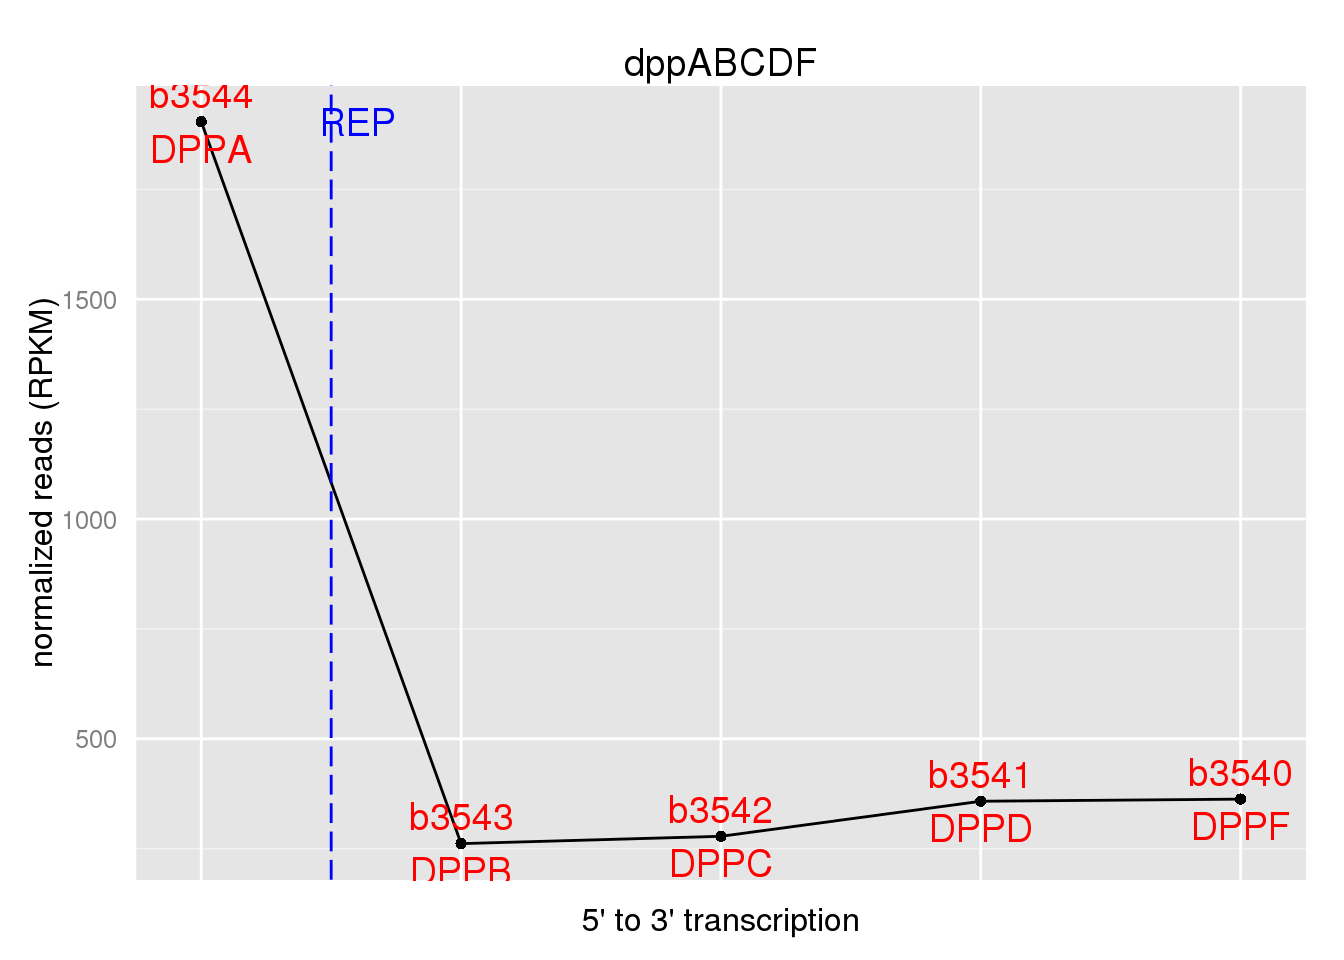
\includegraphics[scale=0.45]{figures/expression1.png}}
\subfigure[Position et organisation de l'opéron, des REP et couverture.]{\label{fig:expressionFigB} 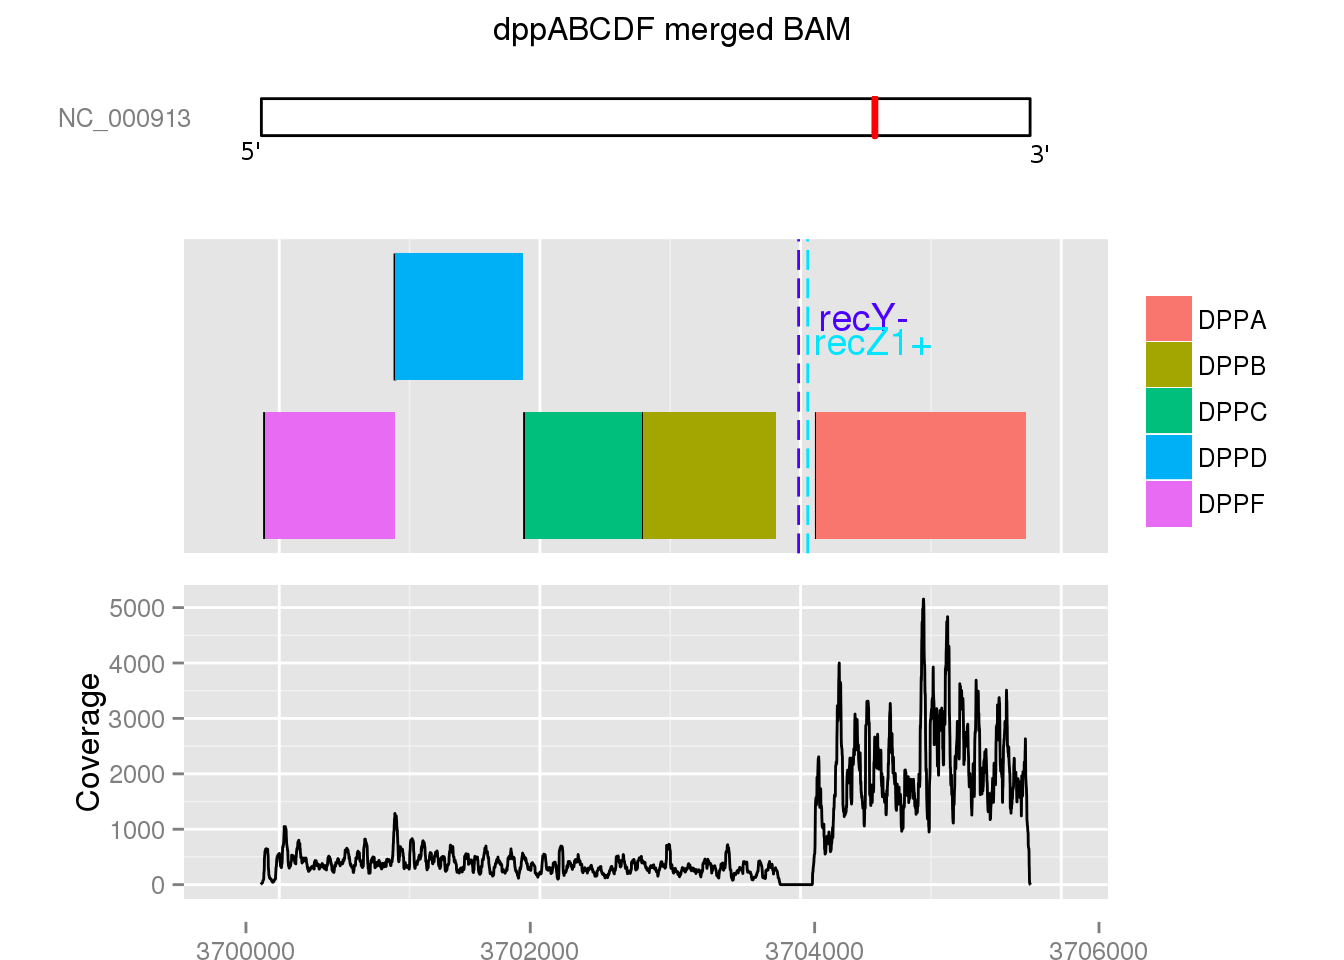
\includegraphics[scale=0.45
]{figures/expression2.png}}
\caption{\textbf{Résultats de l'étude de l'expression des gènes dans les opérons contenant des BIME. (a)} Le taux d'expression de chaque gène de l'opéron est représenté en ordonnées, l'organisation des gènes de l'opéron est schématisée sur l'axe des abscisses dans le sens 5' $\mapsto$ 3'. La position de la ou les REP composant la BIME est schématisée par la ligne bleue verticale. \textbf{(b)} La position de l'opéron sur le génome est indiquée par la barre rouge sur l'idéogramme de la partie supérieure. La partie médiane représente l'organisation des gènes de l'opéron dans le sens 5' $\mapsto$ 3' ainsi que le positionnement et la classe des REP composant la BIME. La partie inférieure montre la couverture par rapport à l'organisation de la partie médiane.}
\label{fig:expression} 
\end{figure}

Pour les gènes dont le test est significatif, deux représentations graphiques sont générées (\autoref{fig:expression}). La 1\up{ère} est un schéma décrivant les niveaux d'expression des gènes de l'opéron ainsi que la position relative des REP formant la BIME (\autoref{fig:expressionFigA}). La 2\up{nde} est une représentation de la couverture sur l'opéron par rapport à l'organisation génomique de celui-ci ainsi que la catégorisation des REP composant la BIME (\autoref{fig:expressionFigB}). Deux fichiers au format \texttt{CSV} sont créés, l'un pour les gènes où nous observons un différence d'expression significative, le second pour les autres cas.

\subsection*{Analyse par corrélation de profils d'expression}
Nous avons développé une méthode réalisant un test de corrélation entre les profils d'expression des régions contenant des BIME et un profil modèle de changement d'expression en nous inspirant d'une technique mise au point pour la prédiction d'opérons dans les génomes bactériens. Le principe général est de délimiter les bornes des transcrits à partir de données de RNA-Seq en s'appuyant sur la corrélation entre le profil d'expression recueilli sur ces données et un profil simulé de 0 et de 1. Les 0 représentant une zone sans couverture donc en dehors d'un transcrit et les 1 la zone couverte, donc le transcrit \citep{Fortino2014}. Pour cela, il a d'abord été nécessaire de délimiter nos régions d'intérêt. Celles-ci se modélisent par la présence du 1\up{er} gène, de la 1\up{ère} région inter-génique, de la BIME, de la 2\up{nde} région inter-génique et du 2\up{nd} gène. Une fois ces régions extraites, le calcul de la couverture base par base a été réalisé à l'aide des BEDtools :
\lstset{language=sh, commentstyle=\color{ForestGreen}}  
\begin{lstlisting}[frame=single]
# Couverture base par base.
bedtools coverage -abam merged.bam -b regionOfInterest.bed \
-d > unsorted_cov_perBase.bed

# Tri en fonction de la position genomique 
# puis de la position des bases dans chaque transcrit
sort -k2 -k7 -n unsorted_cov_perBase.bed | uniq > \
cov_perBase_strandToFix.bed

# Remplacement des '.' par des '*' dans la colonne
# des brins pour l'utilisation sous R
awk 'BEGIN{OFS = "\t"} {gsub(/\./,"*",$6); print }' \
cov_perBase_strandToFix.bed > cov_perBase.bed
\end{lstlisting}

\begin{figure}[ht]
\centerline{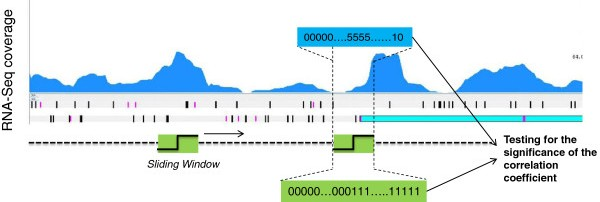
\includegraphics[scale=0.6]{figures/profil.jpg}}
\caption{\textbf{Recherche de corrélation sur des profils d'expression.} La fenêtre glissante (en vert) parcourt la région d'intérêt et pour chaque déplacement une corrélation est calculée entre le vecteur du profil d'expression obtenu par RNAseq (en bleu) et celui simulé par le vecteur de 0 et de 1 (en vert) \citep{Fortino2014}.}
\label{fig:profil} 
\end{figure}

Le cœur de cette méthode consiste déplacer une fenêtre glissante parcourant base à base la région d'intérêt définie ci-dessus en réalisant des tests de corrélation entre le profil d'expression réel et un profil d'expression simulé par un vecteur contenant un nombre égal de 0 et de 1 (si l'on cherche une croissance d'expression en sens ou une décroissance d'expression en anti-sens, e.g: 000111), ou de 1 et de 0 (dans le cas d'une décroissance en sens et d'une croissance en anti-sens, e.g: 111000). Les moyennes d'expression sont récupérées sur les parties gauche et droite de la fenêtre pour dans un premier temps filtrer les données. Le $Log_2$ du rapport de ces moyennes doit être supérieur à un seuil, si ce 1\up{er} filtre est passé, la corrélation entre le profil réel et celui simulé est calculée et doit être supérieure à un seuil avec une p-valeur significative (\autoref{fig:profil}). Les seuils que nous avons fixés sont les suivants : 
\begin{itemize}[label=$\bullet$]
\item fenêtre glissante de 300 bases
\item au moins un des deux gènes possède une couverture > 10
\item $log_2(\frac{\overline{couverture~droite}~+~1}{\overline{couverture~gauche}~+~1})~\geq~1$ pour un profil \_\_\_|\^{ }\^{ }\^{ }
\item $log_2(\frac{\overline{couverture~gauche}~+~1}{\overline{couverture~droite}~+~1})~\geq~1$ pour un profil \^{ }\^{ }\^{ }|\_\_\_
\item une corrélation > 0.7
\item une p-valeur du test de corrélation $< 10^7$
\end{itemize}
\begin{SCfigure}[][t]
\fbox{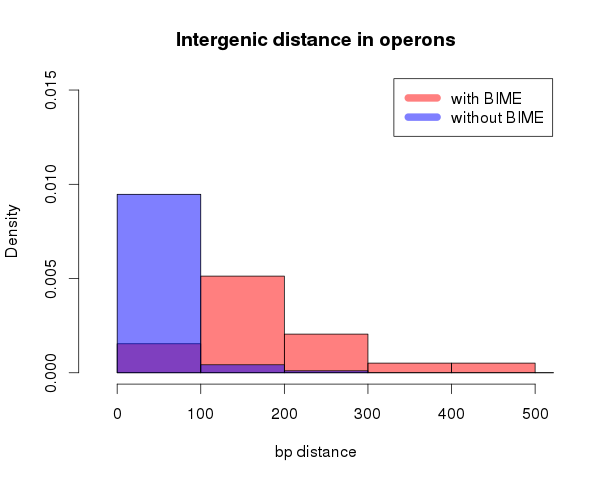
\includegraphics[scale=0.5]{figures/igr_distance.png}
\caption{\textbf{Distances inter-géniques dans les opérons avec et sans BIME.} En bleu absence de BIME dans la région inter-génique, en rouge présence de BIME. Pour les données en absence de BIME, nous observons une valeur modale dans les régions inter-géniques de 50 pb, alors qu'en présence de BIME, la valeur modale se situe dans les régions inter-géniques de 150 pb.}
\label{fig:igr_distance} }
\end{SCfigure}

Le choix de la taille de la fenêtre glissante a été motivé par la taille des régions inter-géniques contenant des BIME dans les opérons . L'idée étant de rechercher le changement d'expression en ayant des informations sur la couverture moyenne des gènes entourant la BIME. La \autoref{fig:igr_distance} nous indique que les majorité des régions contenant des BIME se situent dans les 150 pb. Comme la BIME se situe dans la majorité des cas proche d'un des deux gènes nous avons opté pour une fenêtre de taille 300 pb pour couvrir à la fois les gène et la région inter-génique. Les seuils de corrélation, de p-valeur ont été repris de la publication ainsi que le $Log_2 \geq~1$ représentant un facteur 2 de changement d'expression.

\begin{figure}[ht]
\centerline{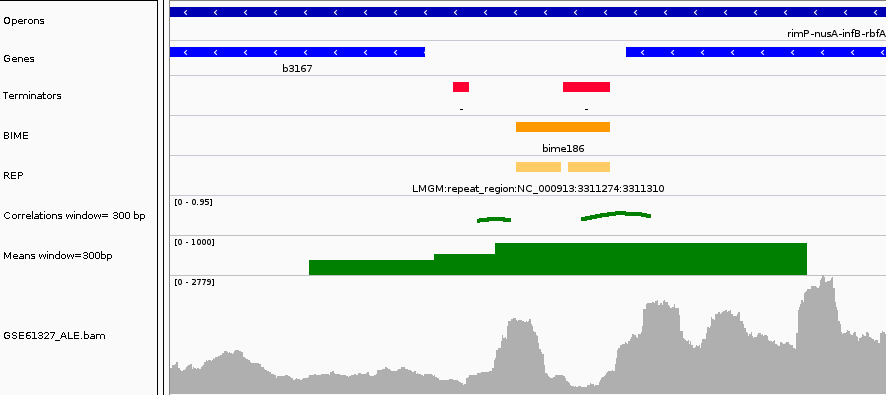
\includegraphics[scale=0.35]{figures/igv_profil.png}}
\caption{\textbf{Visualisation des changements d'expression obtenus par la méthode de corrélation des profils.} La position de la BIME est représentée en orange, le diagramme de barres à 2 colonnes en vert montre les profils d'expression moyens de chaque moitié de la fenêtre et la courbe en points verts indique l'évolution de la corrélation sur cette zone. Dans cet exemple, ce changement d'expression peut se traduire par une augmentation en sens ou une diminution en anti-sens.}
\label{fig:igv_profil} 
\end{figure}

Sur un ensemble de positions consécutives dont les corrélations sont significatives et sont situées sur l'espace génomique de la BIME (étendu de 40 pb de chaque côté), celle dont la corrélation est la plus élevée sera définie comme position de changement d'expression. Deux types de fichiers sont générés au format \texttt{bedgraph} pour une visualisation sur un Genome Browser, le premier sous forme de diagramme de barre représentant les couvertures moyennes des deux parties de la fenêtre, le second représentant l'évolution de la corrélation sur la zone (\autoref{fig:igv_profil}). Une visualisation des niveaux d'expression des 2 gènes et de la BIME est également générée sous forme d'histogrammes avec les informations de sens et du type de la BIME (\autoref{fig:profil_plot}). Finalement, un fichier au format \texttt{CSV} recueille toutes les informations de l'analyse.

\begin{SCfigure}[][t]
\fbox{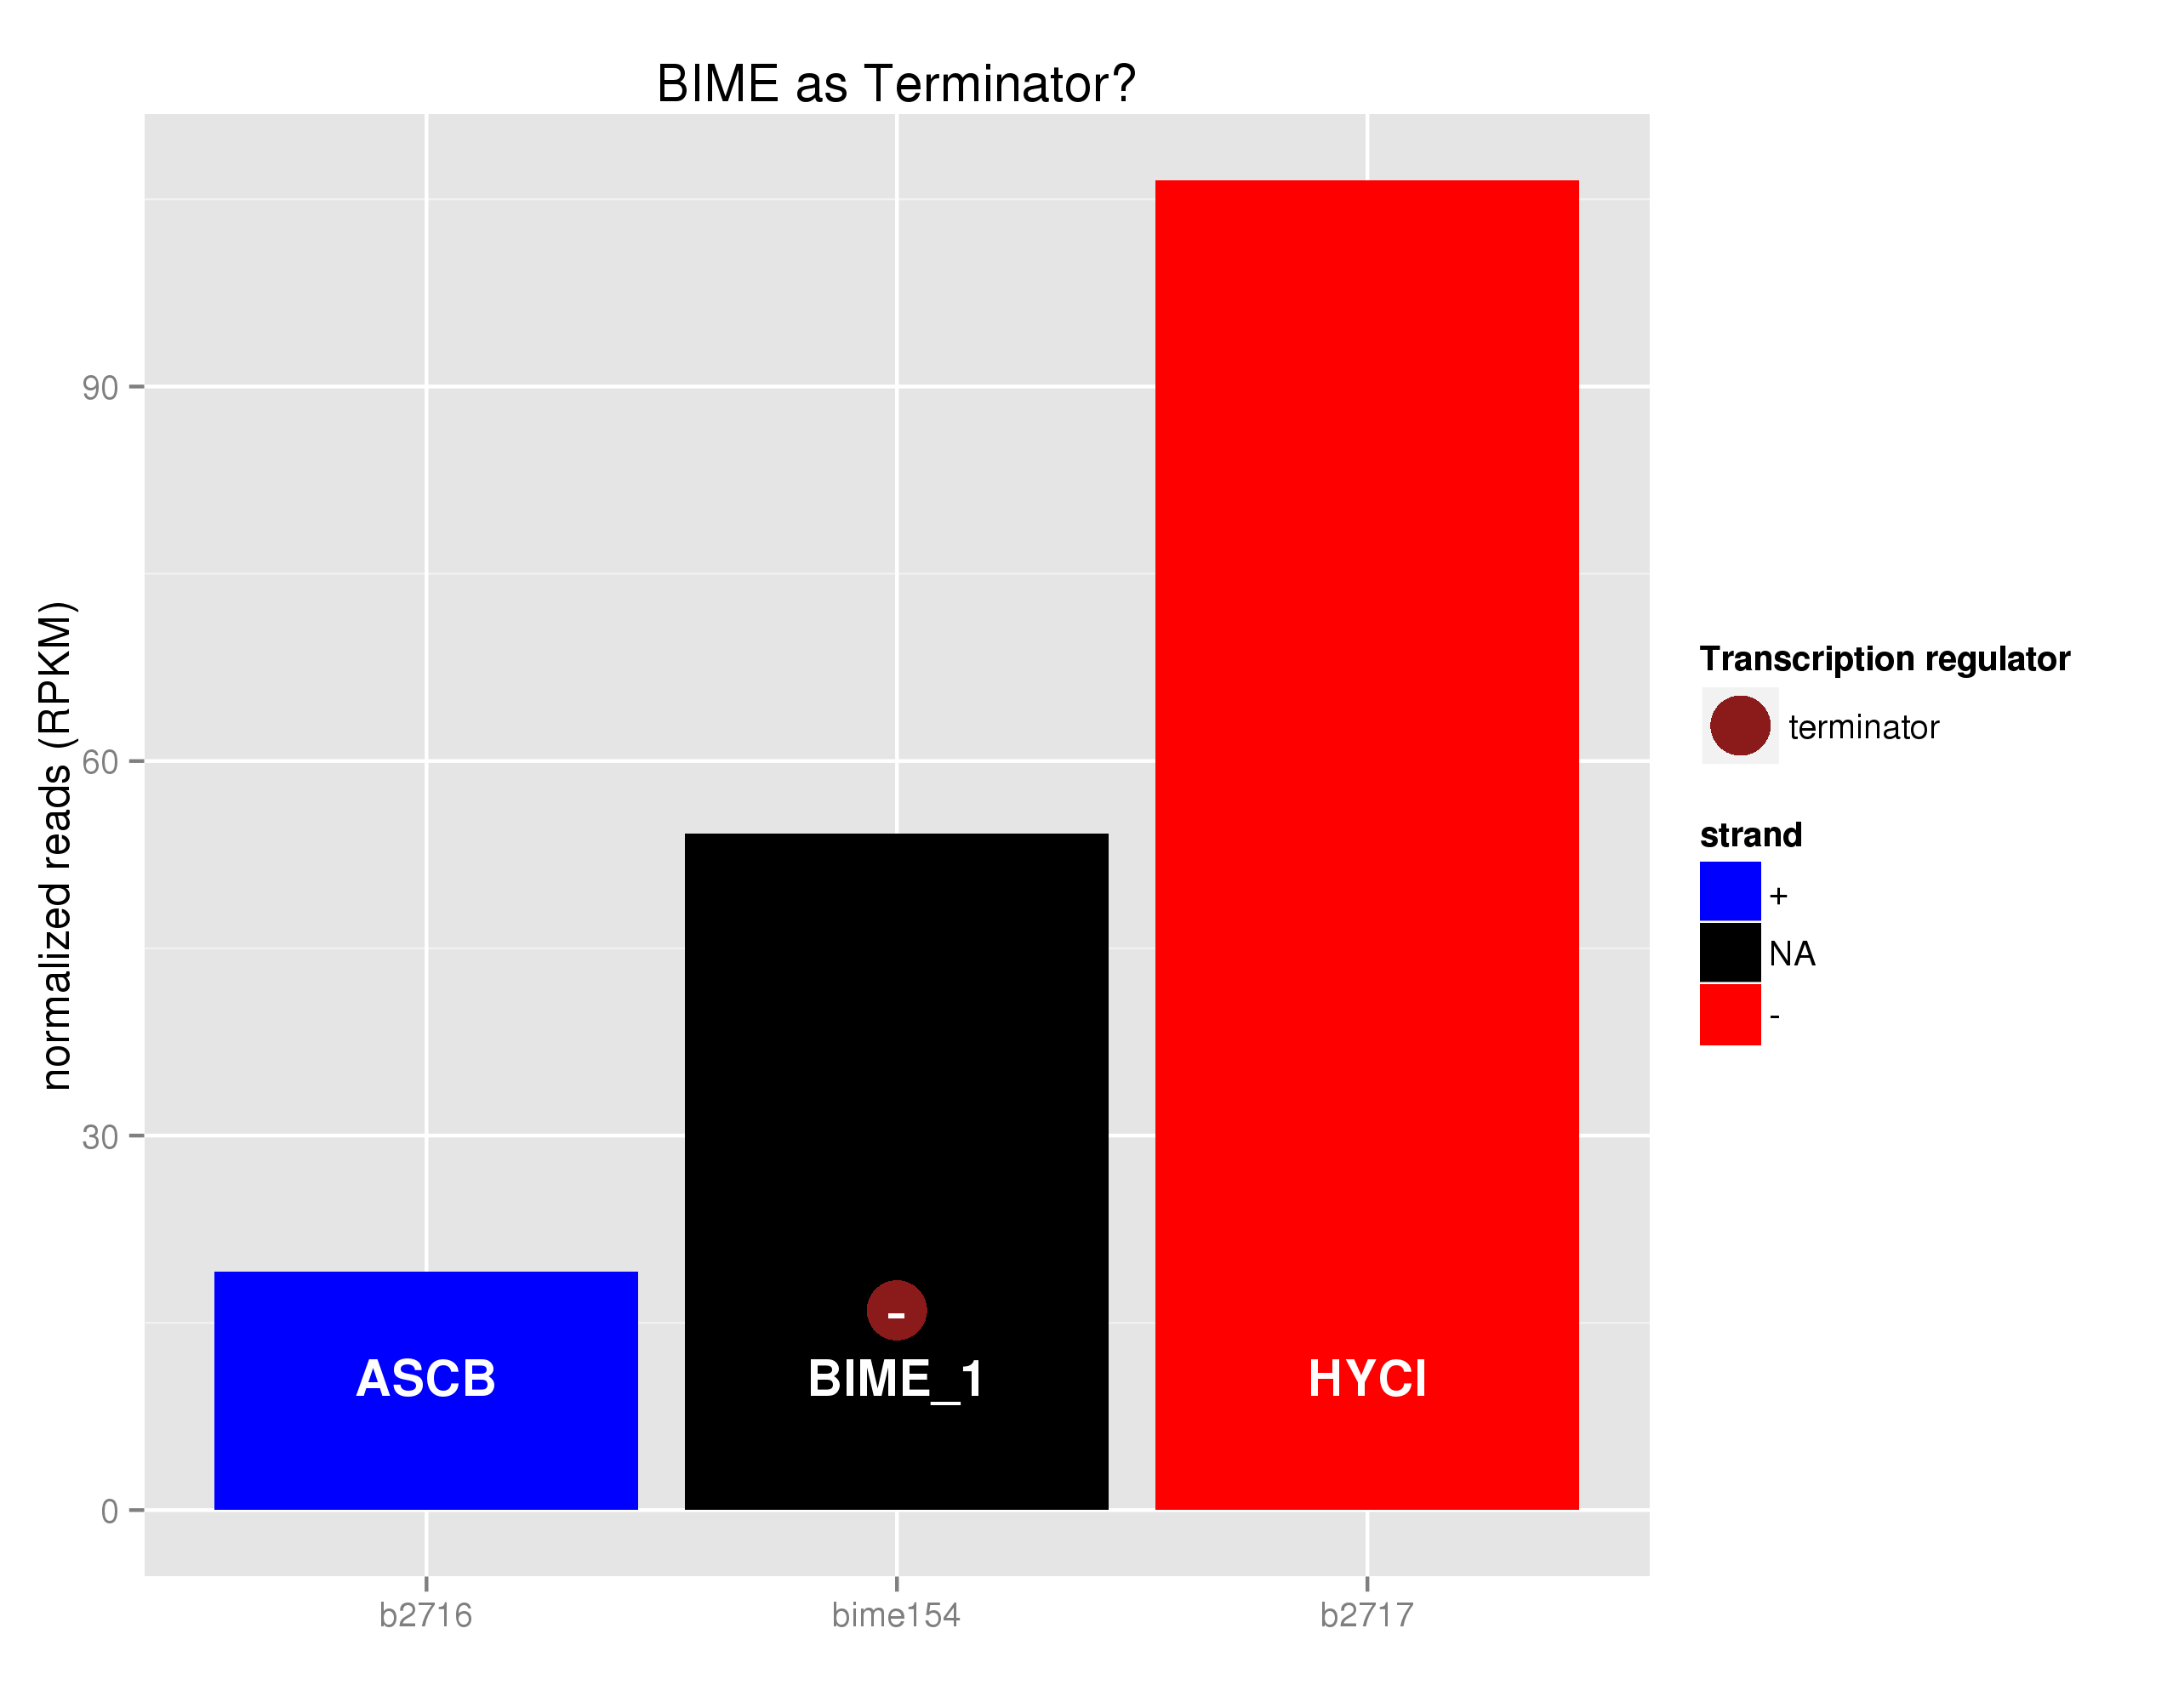
\includegraphics[scale=0.42]{figures/profil_plot.png}
\caption{\textbf{Résultat de corrélation de profils.} Les niveaux d'expression des gènes encadrant la BIME et de cette dernière sont représentés par les histogrammes. La couleur de l'histogramme indique le sens de transcription de l'élément, bleu pour le brin sens, rouge pour l'anti-sens et noir lorsque aucun brin est défini. La présence d'éléments de régulation dans la région inter-génique est représentée par des ronds de couleur verte pour les promoteurs et rouge pour les terminateurs avec un symbole '+' ou '-' pour indiquer le brin de cet élément. La représentation est schématique et ne donne pas d'information sur la position exacte de ces éléments.}
\label{fig:profil_plot} }
\end{SCfigure}

\subsection*{Analyse par segmentation}
A la différence de la méthode précédente, la segmentation ne requière pas l'utilisation de profils. La méthode de segmentation que nous utilisons est issue du package R \href{http://cran.r-project.org/web/packages/Segmentor3IsBack/index.html}{Segmentor3IsBack} \citep{Cleynen2014}. Le but de cette méthode est de rechercher, sur une zone d'intérêt, des points de changements abrupts dans la couverture en utilisant l'algorithme \gls{pdp} \citep{Rigaill2010}. La segmentation se fonde sur le partitionnement d'un signal de $n$ points, la couverture de notre région d'intérêt, compris dans l'ensemble ${\{y_t\}_{t=1,\ldots,n}}$, suivant une distribution de Poisson, en $K$ segments, tel que :
\[ Y_t \sim G(\theta_r) \quad \text{si}\ t \in r \quad \text{et}\ r \in m \]
où $m$ est une partition de $[1,n]$ en $r$ segments, le paramètre $\theta_r$ est la moyenne associée au segment $r$. L'objectif étant d'estimer le point de cassure ou la position des segments et le paramètre $\theta_r$ résultant de la segmentation. $M_{K,n}$ est alors l'ensemble des partitions possibles avec $K$ le nombre minimal de partitions demandé et $n$ la taille de notre région. L'algorithme tente de choisir la partition $M_{K,n}$ avec la perte $\gamma$ minimale. Cette perte est calculée par la négative log-likelihood du modèle. La fonction de calcul du coût est définie comme telle :
\[ c(r,\theta) = \sum_{i \in r} \gamma(y_i,\theta) \]
et dont le coût optimal sera :
\[ c(r) = min_\theta\{c(r,\theta)\} \]
cela permettant de récupérer la segmentation optimale $M_{K,n}$ et son coût $C_{K,n}$. L'algorithme itératif PDP intervient ensuite et est basé sur la minimisation de la fonction de coût $C_{k,t}$ décomposée de la façon suivante :
\begin{equation}
\label{eq1}
C_{k,t} = \underset{\{k-1<\tau<t\}}{min} \{C_{k-1,\tau} + \underset{\theta}{min}[c([\tau + 1,t],\theta)]\}
\end{equation}
où $\theta$ est le paramètre de coût du dernier segment directement lié au calcul de perte $\gamma$. La spécificité de cet algorithme est qu'il s'appuie sur la comparaison de candidats pour la position du dernier point de cassure notée $\tau$ à travers les permutations des minimisations de \eqref{eq1} et avec l'introduction de la fonction :
\[ H_{k,t}(\theta) = \underset{\{k-1<\tau<t\}}{min} \{C_{k-1,\tau} + c([\tau + 1,t],\theta)\} \]
qui est le coût de la meilleur partition en $k$ régions jusqu'à $t$, le paramètre du dernier segment étant $\theta$. $C_{k,t}$ est alors obtenu comme le $min_\theta\{H_{k,t}(\theta)\}$.
Pour chaque itération $k$, l'algorithme travaille sur une liste de candidats pour les derniers points de cassure. Pour chaque élément $\tau$ et chaque valeur $t$, il met à jour un ensemble $S_{k,t}^\tau$ contenant les paramètres $\theta$ pour lequel ce candidat est optimal. Si cet ensemble $S_{k,t}^\tau$ est vide, le candidat est supprimé autorisant un élagage et une diminution de la complexité de l'algorithme.

Au final, l'utilisation de ce package produit un découpage de la région d'intérêt en $K$ segments, $K$ étant fixé par l'utilisateur, dont les limites sont définies par les positions de leurs points de cassures. Nous avons fixé le paramètre $K$ à 4 segments maximum donc 3 points de cassure de façon à vérifier la présence éventuelle de plusieurs de ces points sur la région inter-génique.
Dans notre étude, nous nous intéressons aux positions de ces points de cassures pour nos régions d'intérêt, lorsqu'au moins un des deux gènes possède une couverture supérieure à 10. Les résultats sont croisés avec la présence de promoteurs ou de terminateurs dans la région inter-génique et si les deux gènes appartiennent à un opéron, un test de significativité de la différence d'expression est réalisé avec la même méthodologie que pour la partie~\nameref{subsec:expression}.

\begin{SCfigure}[][t]
\fbox{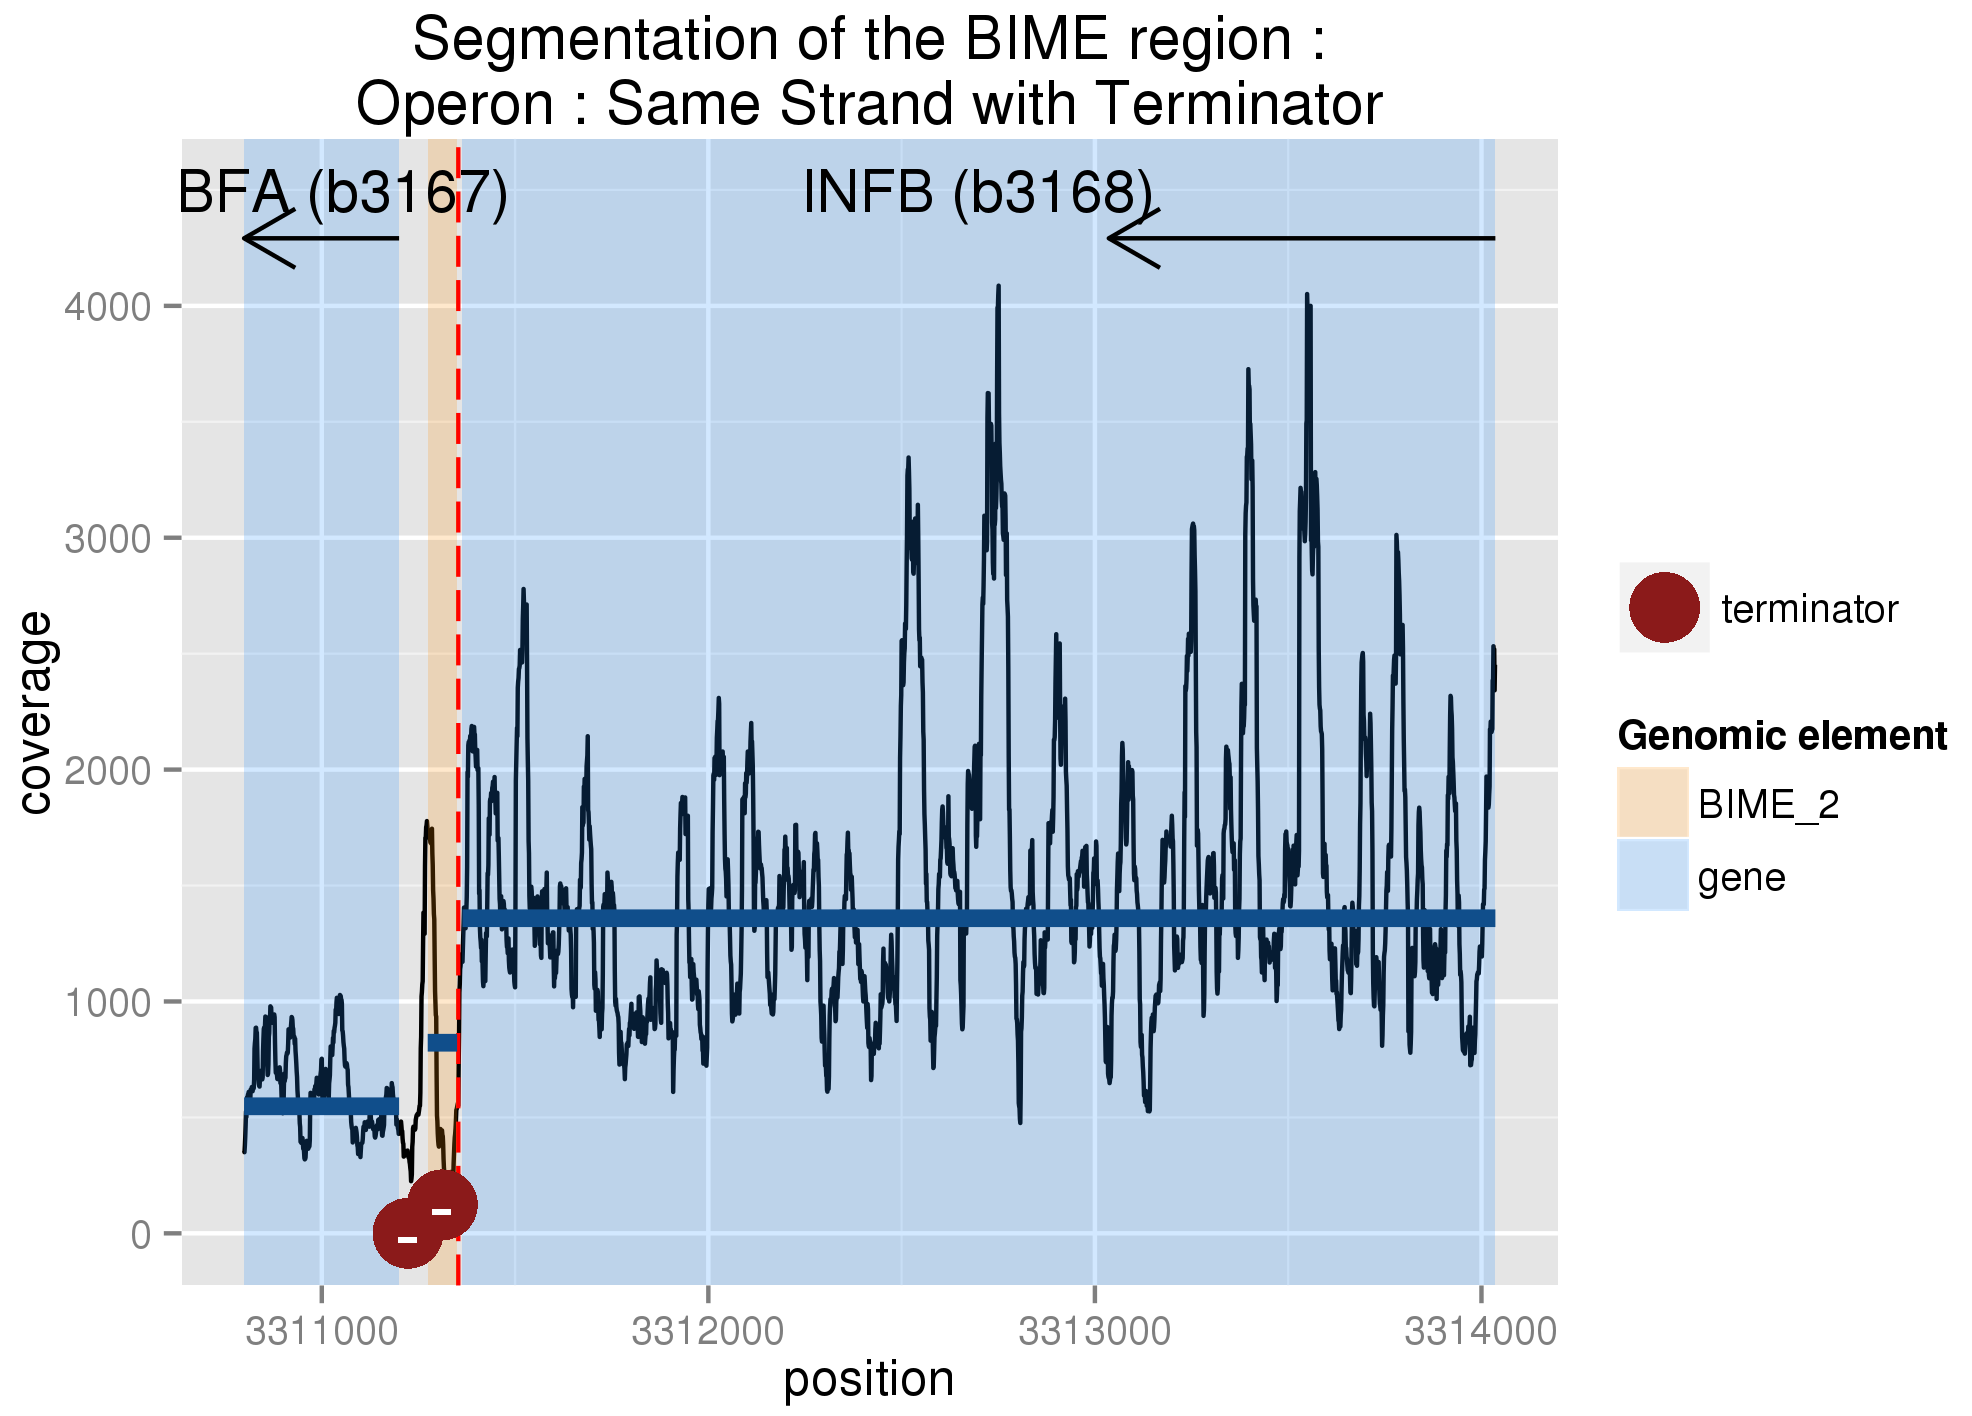
\includegraphics[scale=0.13]{figures/segmentation.png}
\caption{\textbf{Résultat de segmentation pour $K_{max} \mathord{=} 4$.} Les gènes sont symbolisés par les zones bleues, leur sens de transcription par les flèches noires. La BIME est représentée par la zone orange et sa classe est précisée dans la légende (Genomic element). Les promoteurs sont représentés par des points rouges et les terminateurs par des points verts, leur sens affichés par les symboles '+' ou '-' sur ces points. La courbe noire représente la couverture sur la région et les barres bleues horizontales indiquent les couvertures moyennes des éléments génomiques. Les points de cassure dans la couverture, déterminés par la segmentation, sont matérialisés par des lignes rouges verticales en pointillés. Ici, 2 segments sont représentés avec un point de cassure situé en dehors de la BIME après les promoteurs.}
\label{fig:segmentation} }
\end{SCfigure}

L'analyse renvoie une représentation graphique de la couverture de ces régions avec les positionnements des gènes et de la BIME, ainsi que des promoteurs et terminateurs éventuels. Une classification est faite en fonction du sens des gènes et de l'impact des régulateurs de transcription sur la couverture (\autoref{fig:segmentation}). Deux fichiers au format \texttt{CSV} sont générés pour recueillir les informations de la segmentation, le 1\up{er} pour les gènes sur le même brin, le 2\up{nd} pour les gènes sur des brins opposés.

\section*{États ancêtres et structures secondaires}

\chapter*{Résultats}

\chapter*{Discussion}


\end{onehalfspace}


% affichage du glossaire
\renewcommand{\thepage}{}
\printglossary[type=\acronymtype ,title=Glossaire]

%\bibliographystyle{unsrtnat}
\bibliography{biblio_rapport}

\end{document}